The third aspect of the implementation of the site that enables it to contribute to civil society is through the provision of open source, freely available code.

\begin{figure}[h]
  \centering
  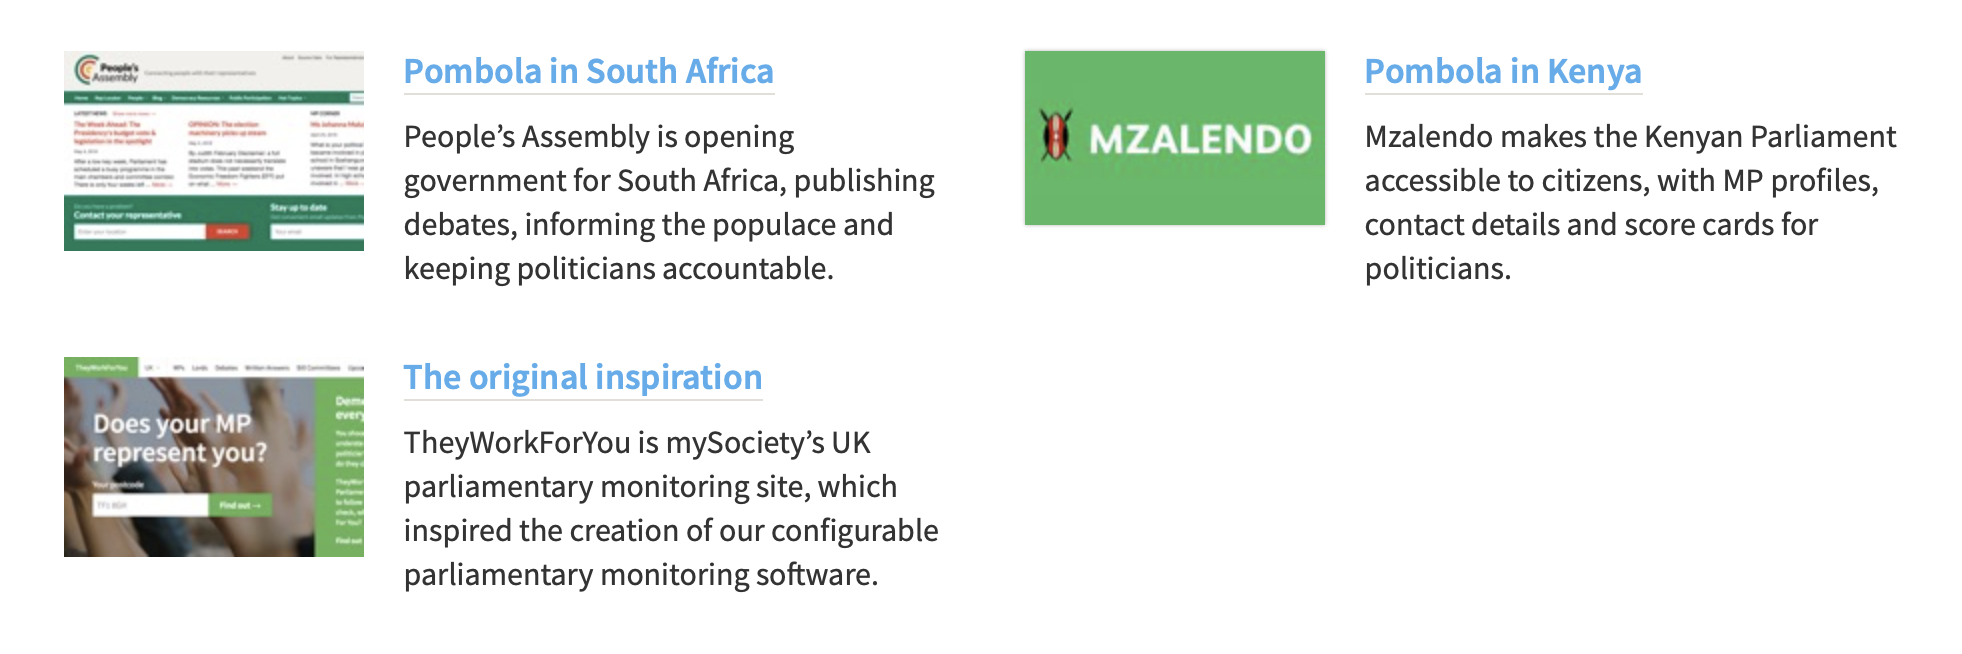
\includegraphics[scale=0.3]{images/they-work-for-you-implementation-open-source-pombola}
  \caption{They Work for You: Pombola}
  \label{fig:they-work-for-you-implementation-open-source-pombola}
\end{figure}

To that end, the They Work for You site was redevloped into into a tool called Pombola.
The screen shot within Figure \ref{fig:they-work-for-you-implementation-open-source-pombola} depicts information about Pombola showing that it is currently being used to provide information about the parliaments in both Kenya and South Africa.

\begin{figure}[h]
  \centering
  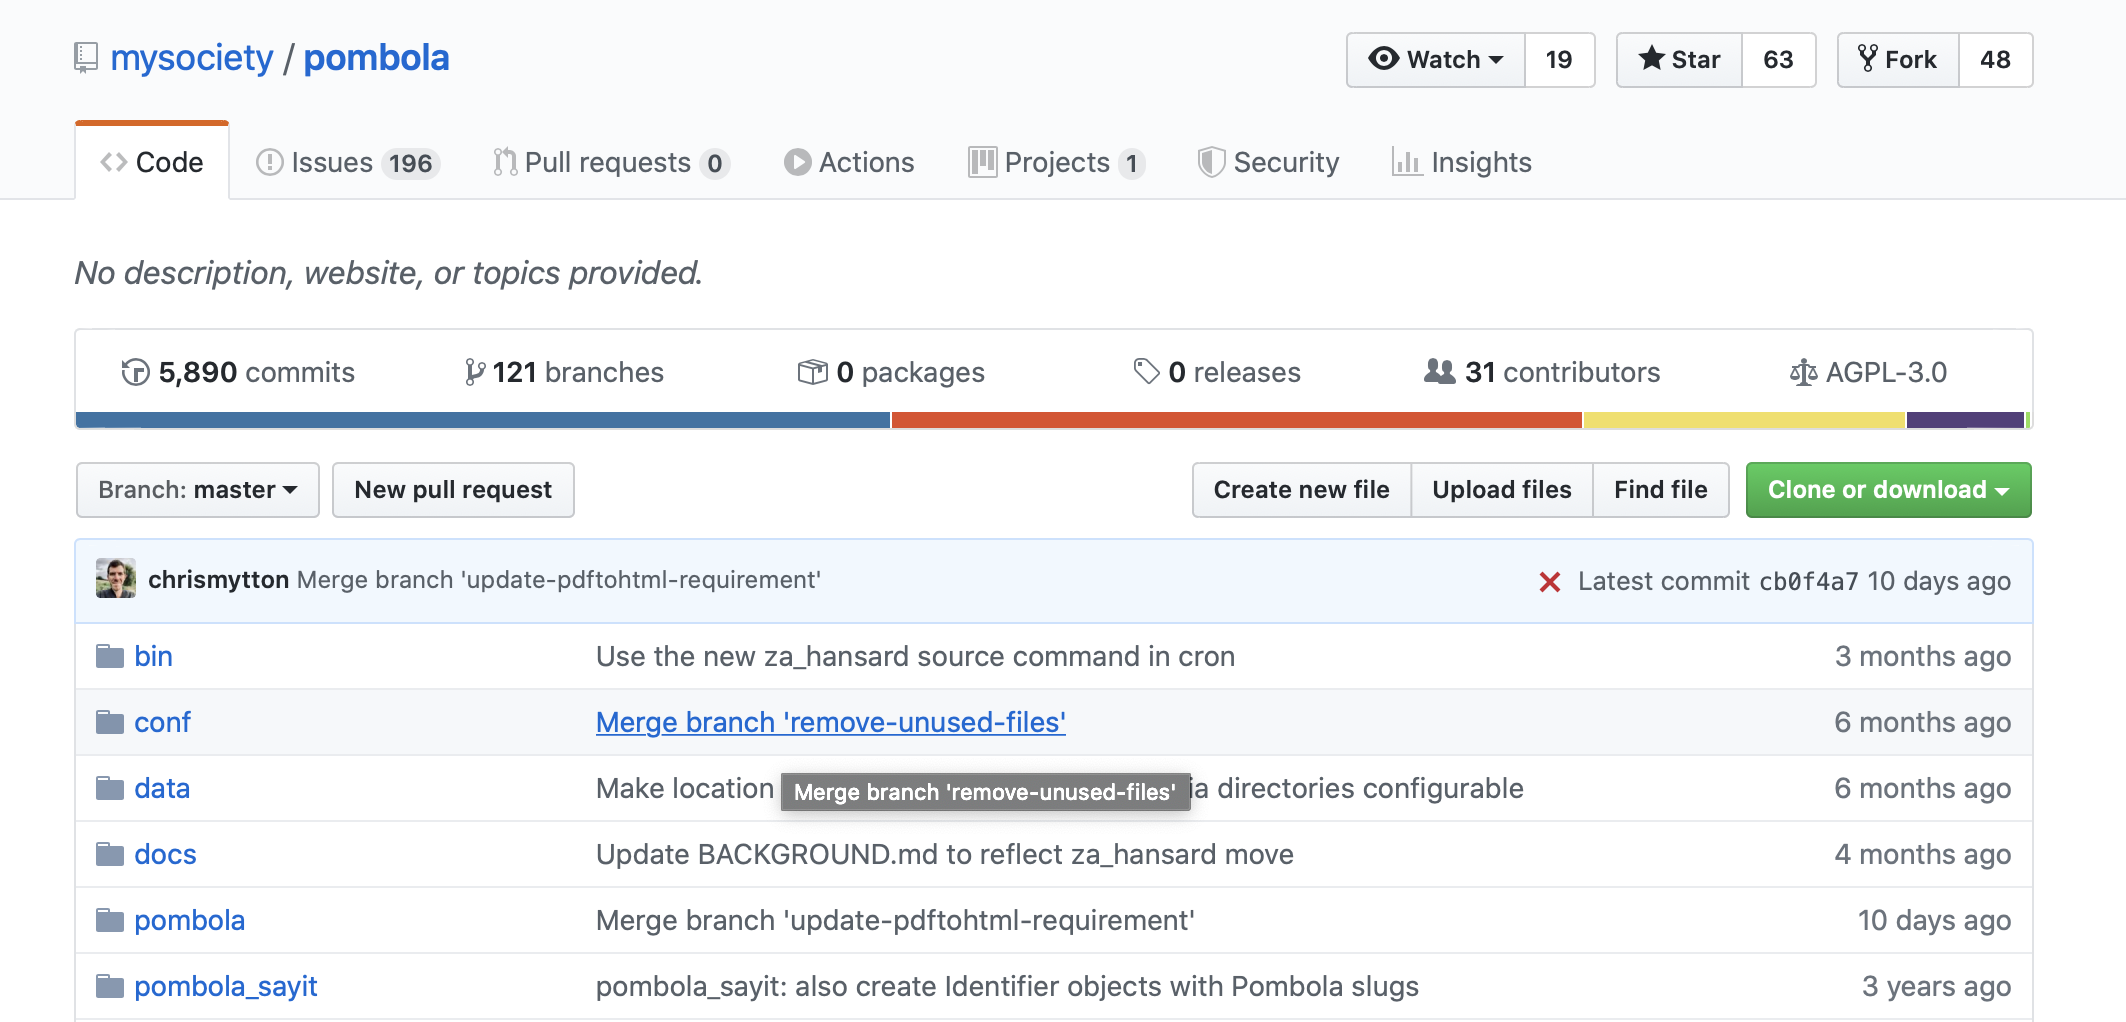
\includegraphics[scale=0.3]{images/they-work-for-you-implementation-open-source-github}
  \caption{They Work for You: GitHub}
  \label{fig:they-work-for-you-implementation-open-source-github}
\end{figure}

The Pombola code \cite{mysociety-github} is freely accessible from the GitHub \cite{github} open source, online code repository, as be seen within Figure \ref{fig:they-work-for-you-implementation-open-source-github}.
It is worth noting that the development of Pombola was financed by the Omidyar Network \cite{omidyar-network}, which is a philanthropic investment organisation, and which was launched by the founder of the aution based e-commerce site eBay \cite{ebay} Pierre Omidyar \cite{pierre-omidyar}.
Furthermore, and highlighting the sometimes complex interplay between civic technologies, the tools that the use, and commercial technologies, GitHub was recenty bought by Microsoft \cite{microsoft-buys-github}.